\documentclass[t]{beamer}
\usetheme{Copenhagen}
\usepackage{amsmath, tikz, pgfplots, array, graphicx}
\tikzset{>=stealth}
\pgfplotsset{compat=newest}
\pgfplotsset{every tick label/.append style={font=\scriptsize}}
\setbeamertemplate{headline}{} % remove toc from headers
\beamertemplatenavigationsymbolsempty
\everymath{\displaystyle}

\title{Graphs of Tangent, Cotangent, Secant, and Cosecant}
\date{}

\AtBeginSection[]
{
  \begin{frame}
    \frametitle{Objectives}
    \tableofcontents[currentsection]
  \end{frame}
}

\begin{document}

\begin{frame}{}
    \maketitle
\end{frame}

\section{Determine the amplitude, period, phase shift, and vertical shift of the tangent and cotangent graphs.}

\begin{frame}{Tangent and Cotangent Graphs}
Recall that $\tan = \frac{y}{x}$. \\[20pt]    \pause

Since $x$- and $y$-coordinates can be positive, negative, or zero, the graphs of tangent and cotangent functions pose some interesting behavior; in particular, when the $x$-coordinate is 0.
\end{frame}

\begin{frame}[c]{Vertical Asymptotes}
    A \alert{vertical asymptote} is a vertical line that the graph will get infinitely close to, but never cross.
\end{frame}

\begin{frame}[c]{Tangent Graph}
\begin{center}
    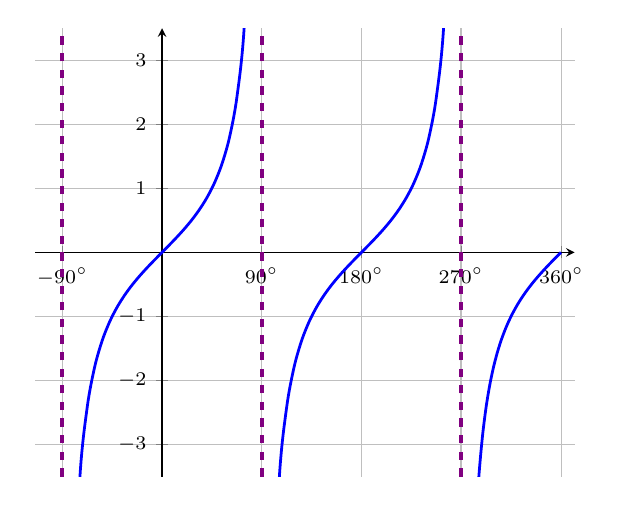
\begin{tikzpicture}
    \begin{axis}[
    axis lines = middle,
    xmin = -2, xmax = 6.5,
    ymin = -3.5, ymax = 3.5,
    grid, domain=0:8.5,
    xtick = {-1.57, 0, 1.57, 3.14, 4.71, 6.29},
    xticklabels = {$-90^\circ$, 0, $90^\circ$, $180^\circ$, $270^\circ$, $360^\circ$},
    xlabel style={at=(current axis.right of origin), anchor=west},
    ytick = {-3,-2,...,3},
    ylabel style={at=(current axis.above origin), anchor=south}
    ]
    \addplot [color=blue, line width = 1, smooth, domain=-0.45*pi:0.45*pi] {tan(deg(x))};
    \addplot [color=blue, line width = 1, smooth, domain=0.55*pi:1.45*pi] {tan(deg(x))};
    \addplot [color=blue, line width = 1, smooth, domain=1.55*pi:2*pi] {tan(deg(x))};
    \addplot [color=violet, line width = 1.5, dashed] coordinates {(-1.57,-3.5) (-1.57,3.5)};
    \addplot [color=violet, line width = 1.5, dashed] coordinates {(1.57,-3.5) (1.57,3.5)};
    \addplot [color=violet, line width = 1.5, dashed] coordinates {(4.71,-3.5) (4.71,3.5)};
    \end{axis}
    \end{tikzpicture}
\end{center}
\end{frame}

\begin{frame}[c]{Cotangent Graphs}
\begin{center}
    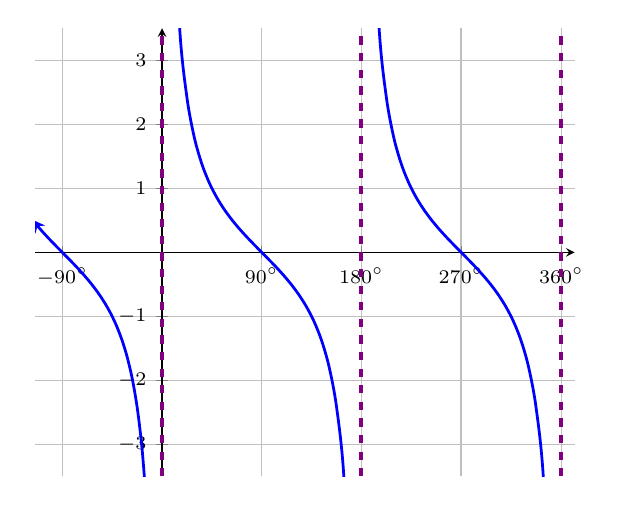
\begin{tikzpicture}
    \begin{axis}[
    axis lines = middle,
    xmin = -2, xmax = 6.5,
    ymin = -3.5, ymax = 3.5,
    grid, domain=0:8.5,
    xtick = {-1.57, 0, 1.57, 3.14, 4.71, 6.29},
    xticklabels = {$-90^\circ$, 0, $90^\circ$, $180^\circ$, $270^\circ$, $360^\circ$},
    xlabel style={at=(current axis.right of origin), anchor=west},
    ytick = {-3,-2,...,3},
    ylabel style={at=(current axis.above origin), anchor=south}
    ]
    \addplot [color=blue, line width = 1, smooth, domain=-0.65*pi:-0.05, <->, >=stealth] {cot(deg(x))};
    \addplot [color=blue, line width = 1, smooth, domain=0.05*pi:0.95*pi] {cot(deg(x))};
    \addplot [color=blue, line width = 1, smooth, domain=1.05*pi:1.95*pi] {cot(deg(x))};
    \addplot [color=violet, line width = 1.5, dashed] coordinates {(0,-3.5) (0,3.5)};
    \addplot [color=violet, line width = 1.5, dashed] coordinates {(3.14,-3.5) (3.14,3.5)};
    \addplot [color=violet, line width = 1.5, dashed] coordinates {(6.29,-3.5) (6.29,3.5)};
    \end{axis}
    \end{tikzpicture}
\end{center}
\end{frame}

\begin{frame}{Amplitude?}
    The graphs of tangent and cotangent functions do not stop going up or down. Thus, they have neither a maximum point nor a minimum point. \newline\\ \pause
    
    In other words, \emph{tangents and cotangents have no amplitude}. 
\end{frame}

\begin{frame}{Period of Tangent and Cotangent}
    Tangents and cotangents complete one full cycle between asymptotes. Notice for each graph, that period is $180^\circ, \text{ or } \pi$ radians. \newline\\ \pause
    
    Like the graphs of sine and cosine, multiplying the inputs, $x$, by a positive value other than 1 will affect the period of the graphs for tangent and cotangent.    \newline\\ \pause 

    Instead of dividing $360^\circ$ (or $2\pi$) by that value, for tangent and cotangent divide $180^\circ$ (or $\pi$ radians).
\end{frame}

\begin{frame}{Shifts}
Determining phase shift and vertical shift follow the same procedures as that for sine and cosine.
\end{frame}

\begin{frame}{Example 1}
Determine the amplitude, period, phase shift, and vertical shift of each of the following.    \newline\\
(a) \quad $y = 2\tan \left(x - 45^\circ \right)$    \newline\\  \pause

Amplitude: None \newline\\  \pause
Period: $\frac{180^\circ}{1} = 180^\circ$
\end{frame}

\begin{frame}{Example 1 \quad $y = 2\tan \left(x - 45^\circ \right)$}
Phase Shift: 
\begin{align*}
    \onslide<2->{x - 45 &= 0} \\
    \onslide<3->{x &= 45}
\end{align*}     \pause
\onslide<4->{Phase Shift: $45^\circ$ right}   \newline\\  
\onslide<5->{Vertical Shift: 0 (or none)}
\end{frame}

\begin{frame}{Example 1}
(b) \quad $y = -\frac{1}{3}\cot x + 1$    \newline\\  \pause
Amplitude: None \newline\\ \pause
Period: $\frac{180^\circ}{1} = 180^\circ$   \newline\\  \pause
Phase Shift: 0 (or none) \newline\\ \pause
Vertical Shift: Up 1
\end{frame}

\begin{frame}{Example 1}
(c) \quad $y = 1.5\tan\left(2x + 120^\circ\right) - 5$  \newline\\ \pause
Amplitude: None \newline\\  \pause
Period: $\frac{180^\circ}{2} = 90^\circ$
\end{frame}

\begin{frame}{Example 1 \quad $y = 1.5\tan\left(2x + 120^\circ\right) - 5$}
Phase Shift:
\begin{align*}
    \onslide<2->{2x + 120 &= 0}   \\
    \onslide<3->{2x &= -120} \\
    \onslide<4->{x &= -60}
\end{align*}
\onslide<5->{Phase Shift: $60^\circ$ left}    \newline\\
\onslide<6->{Vertical Shift: 5 down}
\end{frame}

\section{Determine the amplitude, period, phase shift, and vertical shift of the secant and cosecant graphs.}

\begin{frame}[c]{Secant Graph}
\begin{center}
    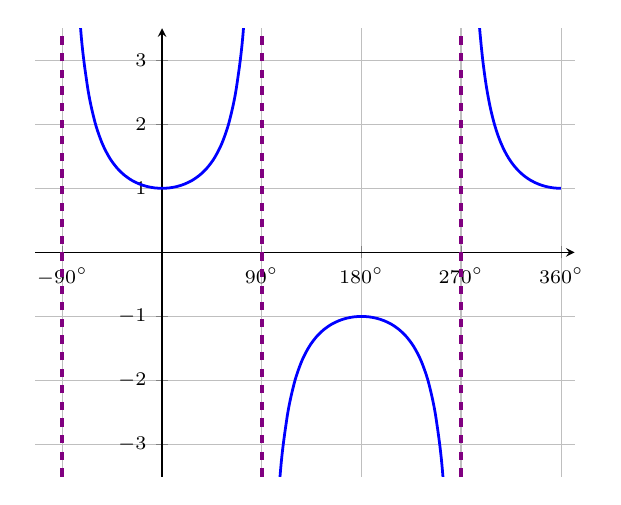
\begin{tikzpicture}
    \begin{axis}[
    axis lines = middle,
    xmin = -2, xmax = 6.5,
    ymin = -3.5, ymax = 3.5,
    grid, domain=0:8.5,
    xtick = {-1.57, 0, 1.57, 3.14, 4.71, 6.29},
    xticklabels = {$-90^\circ$, 0, $90^\circ$, $180^\circ$, $270^\circ$, $360^\circ$},
    xlabel style={at=(current axis.right of origin), anchor=west},
    ytick = {-3,-2,...,3},
    ylabel style={at=(current axis.above origin), anchor=south}
    ]
    \addplot [color=blue, line width = 1, smooth, domain=-0.45*pi:0.45*pi] {sec(deg(x))};
    \addplot [color=blue, line width = 1, smooth, domain=0.55*pi:1.45*pi] {sec(deg(x))};
    \addplot [color=blue, line width = 1, smooth, domain=1.55*pi:2*pi] {sec(deg(x))};
    \addplot [color=violet, line width = 1.5, dashed] coordinates {(-1.57,-3.5) (-1.57,3.5)};
    \addplot [color=violet, line width = 1.5, dashed] coordinates {(1.57,-3.5) (1.57,3.5)};
    \addplot [color=violet, line width = 1.5, dashed] coordinates {(4.71,-3.5) (4.71,3.5)};
    \end{axis}
    \end{tikzpicture} 
\end{center}
\end{frame}

\begin{frame}{Cosecant Graph}
\begin{center}
    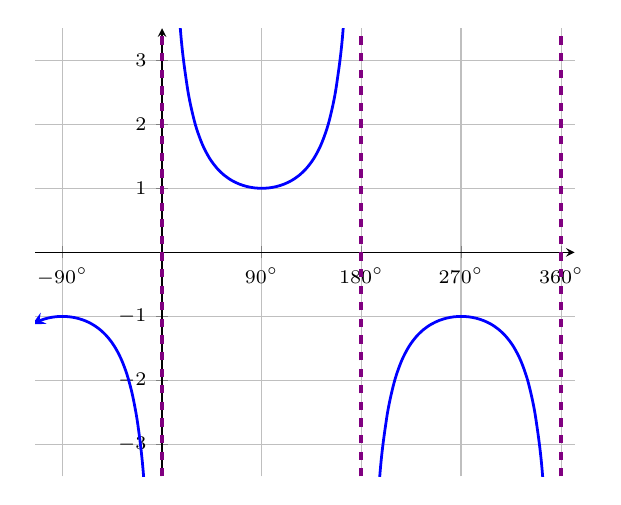
\begin{tikzpicture}
    \begin{axis}[
    axis lines = middle,
    xmin = -2, xmax = 6.5,
    ymin = -3.5, ymax = 3.5,
    grid, domain=0:8.5,
    xtick = {-1.57, 0, 1.57, 3.14, 4.71, 6.29},
    xticklabels = {$-90^\circ$, 0, $90^\circ$, $180^\circ$, $270^\circ$, $360^\circ$},
    xlabel style={at=(current axis.right of origin), anchor=west},
    ytick = {-3,-2,...,3},
    ylabel style={at=(current axis.above origin), anchor=south}
    ]
    \addplot [color=blue, line width = 1, smooth, domain=-0.65*pi:-0.05, <->, >=stealth] {cosec(deg(x))};
    \addplot [color=blue, line width = 1, smooth, domain=0.05*pi:0.95*pi] {cosec(deg(x))};
    \addplot [color=blue, line width = 1, smooth, domain=1.05*pi:1.95*pi] {cosec(deg(x))};
    \addplot [color=violet, line width = 1.5, dashed] coordinates {(0,-3.5) (0,3.5)};
    \addplot [color=violet, line width = 1.5, dashed] coordinates {(3.14,-3.5) (3.14,3.5)};
    \addplot [color=violet, line width = 1.5, dashed] coordinates {(6.29,-3.5) (6.29,3.5)};
    \end{axis}
    \end{tikzpicture}
\end{center}
\end{frame}

\begin{frame}{Relationship to Sine and Cosine}
    If we graph $y = \cos x$ in the same plane as $y = \sec x$, we see some interesting features:
    \begin{center}
    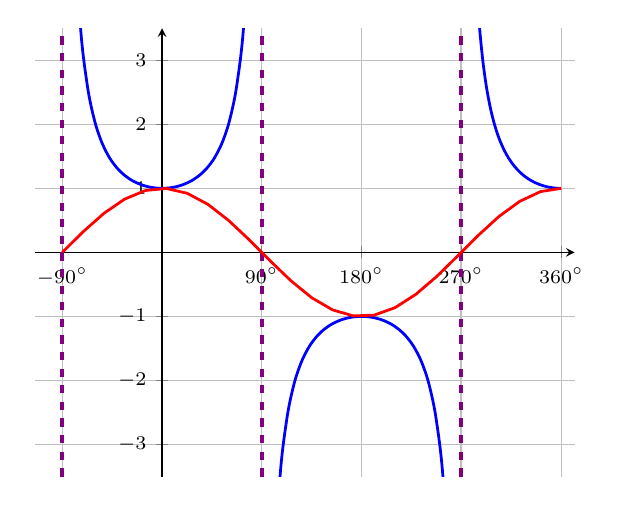
\begin{tikzpicture}
    \begin{axis}[
    axis lines = middle,
    xmin = -2, xmax = 6.5,
    ymin = -3.5, ymax = 3.5,
    grid, domain=0:8.5,
    xtick = {-1.57, 0, 1.57, 3.14, 4.71, 6.29},
    xticklabels = {$-90^\circ$, 0, $90^\circ$, $180^\circ$, $270^\circ$, $360^\circ$},
    xlabel style={at=(current axis.right of origin), anchor=west},
    ytick = {-3,-2,...,3},
    ylabel style={at=(current axis.above origin), anchor=south}
    ]
    \addplot [color=blue, line width = 1, smooth, domain=-0.45*pi:0.45*pi] {sec(deg(x))};
    \addplot [color=blue, line width = 1, smooth, domain=0.55*pi:1.45*pi] {sec(deg(x))};
    \addplot [color=blue, line width = 1, smooth, domain=1.55*pi:2*pi] {sec(deg(x))};
    \addplot [color=violet, line width = 1.5, dashed] coordinates {(-1.57,-3.5) (-1.57,3.5)};
    \addplot [color=violet, line width = 1.5, dashed] coordinates {(1.57,-3.5) (1.57,3.5)};
    \addplot [color=violet, line width = 1.5, dashed] coordinates {(4.71,-3.5) (4.71,3.5)};
    \addplot [color=red, domain=-1.57:6.29, line width=1] {cos(deg(x))};
    \end{axis}
    \end{tikzpicture}
    \end{center}
\end{frame}

\begin{frame}{Cosine and Secant}
Notice that when $\cos x$ is at a maximum, we get a ``smile" on the secant graph, and when $\cos x$ is at a minimum, we get a ``frown" on the secant graph. \newline\\ \pause

Also, whenever $y=\cos x$ crosses the $x$-axis, there is a vertical asymptote for $y=\sec x$ (why?)   \newline\\ \pause

The same logic applies with $y=\csc x$ and $y=\sin x$.
\end{frame}

\begin{frame}{Sine and Cosecant}
    \begin{center}
    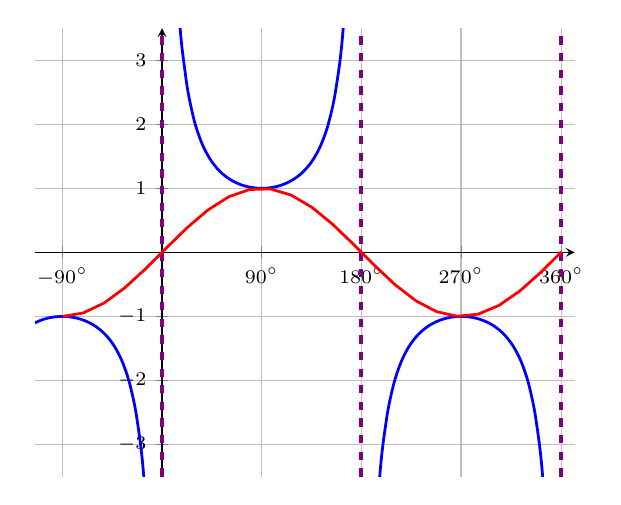
\begin{tikzpicture}
    \begin{axis}[
    axis lines = middle,
    xmin = -2, xmax = 6.5,
    ymin = -3.5, ymax = 3.5,
    grid, domain=0:8.5,
    xtick = {-1.57, 0, 1.57, 3.14, 4.71, 6.29},
    xticklabels = {$-90^\circ$, 0, $90^\circ$, $180^\circ$, $270^\circ$, $360^\circ$},
    xlabel style={at=(current axis.right of origin), anchor=west},
    ytick = {-3,-2,...,3},
    ylabel style={at=(current axis.above origin), anchor=south}
    ]
    \addplot [color=blue, line width = 1, smooth, domain=-0.95*pi:-0.05*pi] {cosec(deg(x))};
    \addplot [color=blue, line width = 1, smooth, domain=0:0.95*pi] {cosec(deg(x))};
    \addplot [color=blue, line width = 1, smooth, domain=1.05*pi:1.95*pi] {cosec(deg(x))};
    \addplot [color=blue, line width = 1, smooth, domain=2.05*pi:2.95*pi] {cosec(deg(x))};
    \addplot [color=violet, line width = 1.5, dashed] coordinates {(0,-3.5) (0,3.5)};
    \addplot [color=violet, line width = 1.5, dashed] coordinates {(3.14,-3.5) (3.14,3.5)};
    \addplot [color=violet, line width = 1.5, dashed] coordinates {(6.28,-3.5) (6.28,3.5)};
    \addplot [color=red, domain=-1.57:6.29, line width=1] {sin(deg(x))};
    \end{axis}
    \end{tikzpicture}
    \end{center}
\end{frame}

\begin{frame}{Properties}
Once again, since there are no maximum nor minimum points, secant and cosecant do not have an amplitude.   \newline\\ \pause

The period of the graphs of secant and cosecant can be found by determining how long it takes one full smile and one full frown to appear. \newline\\ \pause 

From the graphs, we can see that it is $360^\circ$, or $2\pi$ radians (just like sine and cosine).  \newline\\ \pause  

Multiplying the inputs by a positive value other than 1 changes the period. \newline\\ \pause 

Phase shifts and vertical shifts are calculated in the same way as the other four trig functions.
\end{frame}

\begin{frame}{Example 2}
the amplitude, period, phase shift, and vertical shift for each of the following.   \newline\\
(a) \quad $y = 2\sec \left(x - 45^\circ \right)$    \newline\\  \pause
Amplitude: None \newline\\  \pause
Period: $\frac{360^\circ}{1} = 360^\circ$
\end{frame}

\begin{frame}{Example 2 \quad $y = 2\sec \left(x - 45^\circ \right)$}
Phase Shift:    
\begin{align*}
    \onslide<2->{x - 45 &= 0} \\
    \onslide<3->{x &= 45} \\
\end{align*}
\onslide<4->{Phase Shift: $45^\circ$ right} \newline\\ \pause
\onslide<5->{Vertical Shift: 0 (or none)} 
\end{frame}

\begin{frame}{Example 2}
(b) \quad $y = -\frac{1}{3}\csc x + 1$  \newline\\  \pause
Amplitude: None \newline\\ \pause
Period: $\frac{360^\circ}{1} = 360^\circ$   \newline\\  \pause
Phase Shift: None   \newline\\  \pause
Vertical Shift: Up 1
\end{frame}

\begin{frame}{Example 3}
(c) \quad $y = 1.5\csc\left(2x + 120^\circ\right) - 5$  \newline\\  \pause
Amplitude: None \newline\\  \pause
Period: $\frac{360^\circ}{2} = 180^\circ$
\end{frame}

\begin{frame}{Example 3 \quad }$y = 1.5\csc\left(2x + 120^\circ\right) - 5$
Phase Shift:
\begin{align*}
    \onslide<2->{2x + 120 &= 0} \\
    \onslide<3->{2x &= -120} \\
    \onslide<4->{x &= -60}  \\
\end{align*}
\onslide<5->{Phase Shift: $60^\circ$ left} \newline\\
\onslide<6->{Vertical Shift: 5 down}
\end{frame}

\begin{frame}[c]{Summary}
\begin{center}
\setlength{\extrarowheight}{11pt}
\scalebox{0.8}{
\begin{tabular}{|c|c|c|c|c|}
    \hline
    &   \textbf{Amplitude}  &   \textbf{Period} &   \textbf{Phase Shift}  &   \textbf{Vertical Shift} \\[6pt] \hline
    $y=A\tan(Bx-C)+D$   &   None    &   $\dfrac{180^\circ}{B} \text{ or } \dfrac{\pi}{B}$   &  
    $\dfrac{C}{B}$  &   $D$ \\[11pt]  \hline
    
    $y=A\cot(Bx-C)+D$   &   None    &   $\dfrac{180^\circ}{B} \text{ or } \dfrac{\pi}{B}$   &  
    $\dfrac{C}{B}$  &   $D$ \\[11pt]  \hline
    
    $y=A\sec(Bx-C)+D$   &   None    &   $\dfrac{360^\circ}{B} \text{ or } \dfrac{2\pi}{B}$   &  
    $\dfrac{C}{B}$  &   $D$ \\[11pt]  \hline
    
    $y=A\csc(Bx-C)+D$   &   None    &   $\dfrac{360^\circ}{B} \text{ or } \dfrac{2\pi}{B}$   &  
    $\dfrac{C}{B}$  &   $D$ \\[11pt]  \hline
\end{tabular}}
\end{center}
\end{frame}


\end{document}


